\begin{Schunk}
\begin{Sinput}
> library("Ham94", lib.loc = "../../../library")
\end{Sinput}
\end{Schunk}
Pages 50 to 59 describe the calculation of autocorrelation functions of AR and MA processes.
Following the expressions in the text we can calculate results using separate formulae for white
noise, moving average, and autoregressive processes.
\begin{Schunk}
\begin{Sinput}
> T <- 20
> specifications <- list(list(label = "White Noise", MA = vector(mode = "numeric"), 
+     AR = vector(mode = "numeric")), list(label = "MA(1)", MA = c(0.8), 
+     AR = vector(mode = "numeric")), list(label = "MA(4)", MA = c(-0.6, 
+     0.5, -0.5, 0.3), AR = vector(mode = "numeric")), list(label = "AR(1) with 0.8", 
+     MA = vector(mode = "numeric"), AR = c(0.8)), list(label = "AR(1) with -0.8", 
+     MA = vector(mode = "numeric"), AR = c(-0.8)))
> sigmasq <- 1
\end{Sinput}
\end{Schunk}
White noise calculations are described on bottom of page 47 and the top of page 48.
\begin{Schunk}
\begin{Sinput}
> specifications[[1]]$rho <- c(1, rep(0, T - 1))
\end{Sinput}
\end{Schunk}
Moving average calculations are described on page 51.
\begin{Schunk}
\begin{Sinput}
> for (i in 2:3) {
+     MA <- specifications[[i]]$MA
+     q <- length(MA)
+     gamma <- vector(mode = "numeric", length = T)
+     gamma[1] <- sigmasq * t(c(1, MA)) %*% c(1, MA)
+     for (j in 1:q) gamma[j + 1] <- sigmasq * t(MA[j:q]) %*% c(1, 
+         MA)[1:(q - j + 1)]
+     gamma[(q + 2):T] <- 0
+     specifications[[i]]$rho <- gamma/gamma[1]
+ }
\end{Sinput}
\end{Schunk}
Autocorrelation calculations are described on page 59
\begin{Schunk}
\begin{Sinput}
> for (i in 4:5) {
+     AR <- specifications[[i]]$AR
+     p <- length(AR)
+     F <- rbind(AR, cbind(diag(p - 1), rep(0, p - 1)))
+     gamma <- vector(mode = "numeric", length = T)
+     gamma[1:p] <- sigmasq * solve(diag(p^2) - F %x% F)[1:p, 1]
+     for (j in (p + 1):T) gamma[[j]] <- t(gamma[(j - 1):(j - p)]) %*% 
+         AR
+     specifications[[i]]$rho <- gamma/gamma[1]
+ }
\end{Sinput}
\end{Schunk}
\begin{center}
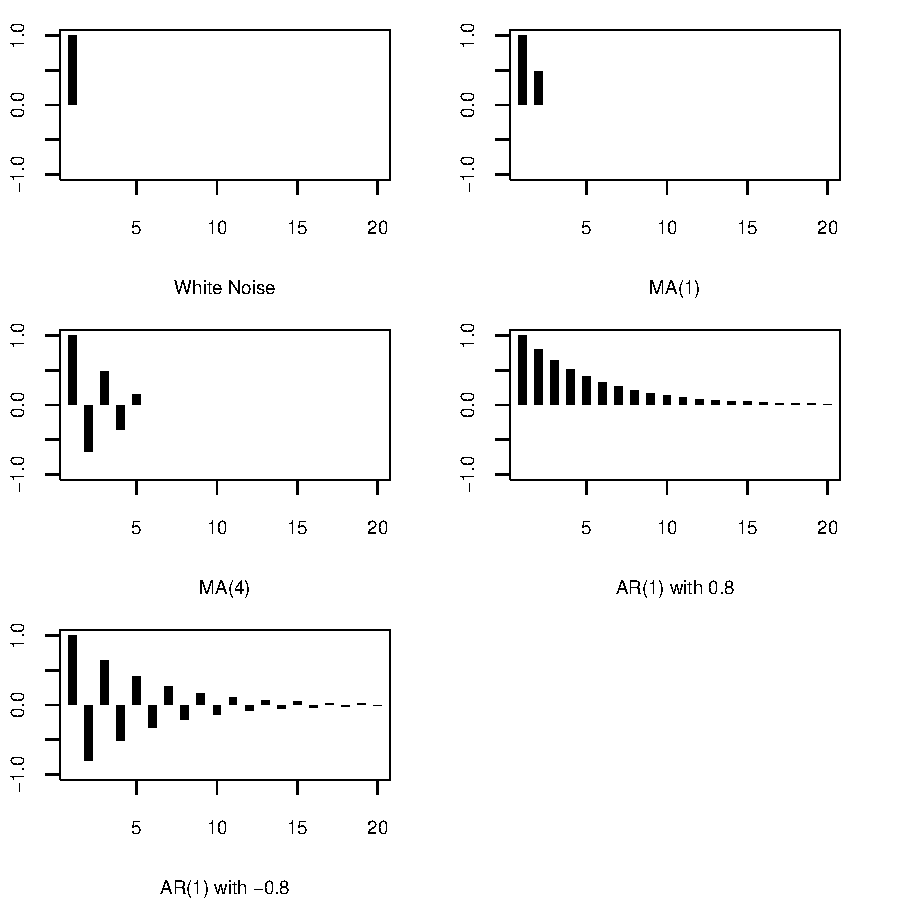
\includegraphics{p50-006}
\end{center}
\subsection{R Facilities for ARMA Autocorrelations}
Function ARMAacf can be used to calculate autocorrelations for an arbitrary ARMA process.
\begin{Schunk}
\begin{Sinput}
> g3 <- ARMAacf(ar = numeric(0), ma = specifications[[3]]$MA, lag.max = T, 
+     pacf = FALSE)
> print(specifications[[3]]$rho)
\end{Sinput}
\begin{Soutput}
 [1]  1.0000000 -0.6666667  0.4871795 -0.3487179  0.1538462  0.0000000
 [7]  0.0000000  0.0000000  0.0000000  0.0000000  0.0000000  0.0000000
[13]  0.0000000  0.0000000  0.0000000  0.0000000  0.0000000  0.0000000
[19]  0.0000000  0.0000000
\end{Soutput}
\begin{Sinput}
> print(g3)
\end{Sinput}
\begin{Soutput}
         0          1          2          3          4          5          6 
 1.0000000 -0.6666667  0.4871795 -0.3487179  0.1538462  0.0000000  0.0000000 
         7          8          9         10         11         12         13 
 0.0000000  0.0000000  0.0000000  0.0000000  0.0000000  0.0000000  0.0000000 
        14         15         16         17         18         19         20 
 0.0000000  0.0000000  0.0000000  0.0000000  0.0000000  0.0000000  0.0000000 
\end{Soutput}
\begin{Sinput}
> g4 <- ARMAacf(ar = specifications[[4]]$AR, ma = numeric(0), lag.max = T - 
+     1, pacf = FALSE)
> print(specifications[[4]]$rho)
\end{Sinput}
\begin{Soutput}
 [1] 1.00000000 0.80000000 0.64000000 0.51200000 0.40960000 0.32768000
 [7] 0.26214400 0.20971520 0.16777216 0.13421773 0.10737418 0.08589935
[13] 0.06871948 0.05497558 0.04398047 0.03518437 0.02814750 0.02251800
[19] 0.01801440 0.01441152
\end{Soutput}
\begin{Sinput}
> print(g4)
\end{Sinput}
\begin{Soutput}
         0          1          2          3          4          5          6 
1.00000000 0.80000000 0.64000000 0.51200000 0.40960000 0.32768000 0.26214400 
         7          8          9         10         11         12         13 
0.20971520 0.16777216 0.13421773 0.10737418 0.08589935 0.06871948 0.05497558 
        14         15         16         17         18         19 
0.04398047 0.03518437 0.02814750 0.02251800 0.01801440 0.01441152 
\end{Soutput}
\end{Schunk}
